\documentclass[11pt]{article}
\usepackage{graphicx}
\usepackage[utf8]{inputenc}
\usepackage{enumerate}
\usepackage{multirow,tabularx}
\usepackage{caption}
\usepackage{subfigure}
\usepackage[T1]{fontenc}
\usepackage{mathptmx}
\usepackage[a4paper, left=2cm, right=2cm, top=2.5cm, bottom=2.5cm, headsep=1.2cm]{geometry} 
\usepackage[rightcaption]{sidecap}
\usepackage{float}
\usepackage{pgfplots}
\pgfplotsset{compat=1.14}
\begin{document}

\begin{titlepage}

	\begin{center}

    


	\huge{\textsc{Metody Komputerowe w Spalaniu}} \\
[50mm]

    \LARGE{\textbf{Premixed flat flame simulation.
}} \\
	[50mm]
	\Large{Norbert Czarnota}\\
    \Large{271292}\\
    [25mm]
    \large{Aerospace Engineering}\\
    [80mm]
    \large{Warsaw, 26.06.2017}\\
    \end{center}
    
\end{titlepage}

\newpage



\section{Purpose of the project}
The purpose of the project is to make a simulation of 1d flame in Cantera (an open source chemical/kinetics software) under different initial temperature and pressure. 
Combustion reaction of the hydrogen with oxygen.



Combustion reaction of hydrogen - oxygen mixture at stoichiometry (and with fi = 0,5 and fi =2):
\begin{displaymath}
2 H_{2} + O_{2}  \Rightarrow  2 H_{2}O 
\end{displaymath}

\section{Mathematical model}
In project I use a premixed mixture of hydrogen and oxygen, I set flame with FreeFlame class (set random real criteria which defined it). As transport criteria I used multicomponent method. I made several calculation at different initial temperature and pressure and then check the results with experiments (see References at the end of raport).

\section{Results and plots}
Where:\\
[2mm]
•	T [K] is temperature during the combustion,\\
[2mm]
•	z [m] is point of the length of the flame,\\
[2mm]
•	Tint [K] is initial temperature,\\
[2mm]
•	pint [Pa] is initial pressure.\\
[2mm]
•	fi – stoichiometry rate
\begin{figure} [H]
	\begin{center}
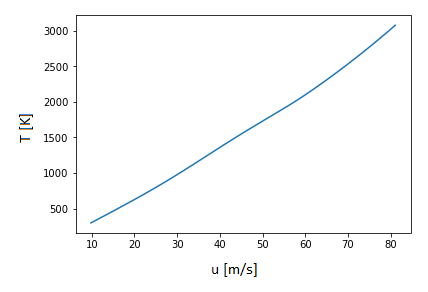
\includegraphics[height=0.5\textwidth]{P1}
        \caption{T [K] (u) [m/s] plot Tint=300K, pint = 1 atm.}
    \end{center}
\end{figure}

\begin{figure} [H]
	\begin{center}
    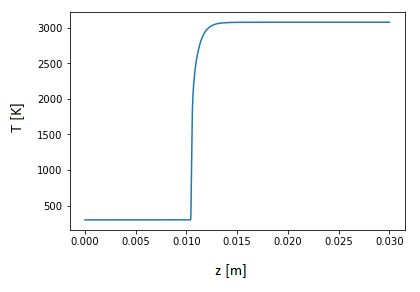
\includegraphics[height=0.5\textwidth]{P2}
        \caption{T (z) [m] plot for Tint = 300K, pint =1 atm.}
    \end{center}
\end{figure}

\begin{figure} [H]
	\begin{center}
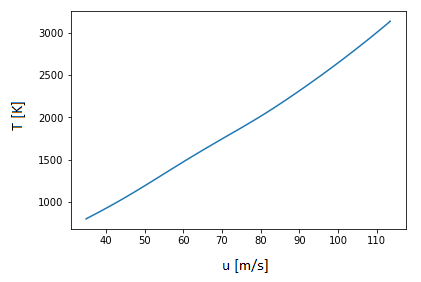
\includegraphics[height=0.5\textwidth]{P3}
        \caption{T (u) plot for Tint=800K, pint = 1 atm.}
    \end{center}
\end{figure}

\begin{figure} [H]
	\begin{center}
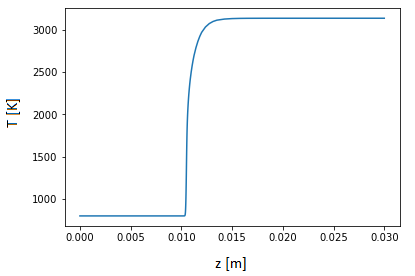
\includegraphics[height=0.5\textwidth]{P4}
        \caption{T (z) plot for Tint=800K, pint = 1 atm.}
    \end{center}
\end{figure}

\begin{figure} [H]
	\begin{center}
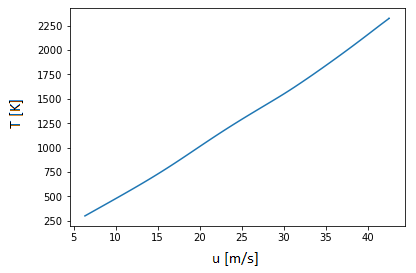
\includegraphics[height=0.5\textwidth]{P5}
        \caption{T (u) plot for Tint=300K, pint = 0,1 atm.}
    \end{center}
\end{figure}

\begin{figure} [H]
	\begin{center}
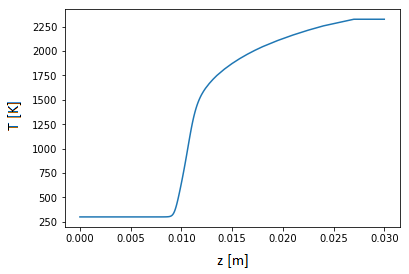
\includegraphics[height=0.5\textwidth]{P6}
        \caption{T (z) plot for Tint = 300K, pint = 0,1 atm.}
    \end{center}
\end{figure}

\begin{figure} [H]
	\begin{center}
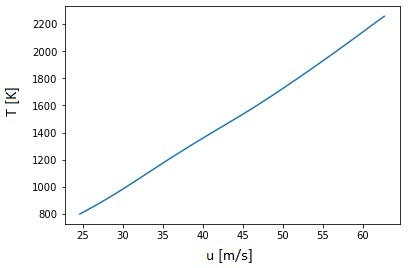
\includegraphics[height=0.5\textwidth]{P7}
        \caption{T (u) plot for Tint=800K, pint = 0,1 atm.}
    \end{center}
\end{figure}

\begin{figure} [H]
	\begin{center}
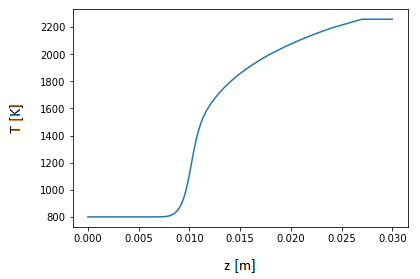
\includegraphics[height=0.5\textwidth]{P8}
        \caption{T (z) plot for Tint = 800K, pint = 0,1 atm.}
    \end{center}
\end{figure}

\begin{figure} [H]
	\begin{center}
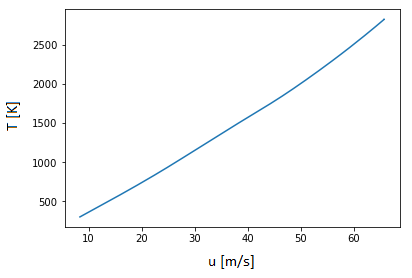
\includegraphics[height=0.5\textwidth]{P9}
        \caption{T (u) plot for Tint = 300 K, pint = 1 atm, fi = 0,5.}
    \end{center}
\end{figure}

\begin{figure} [H]
	\begin{center}
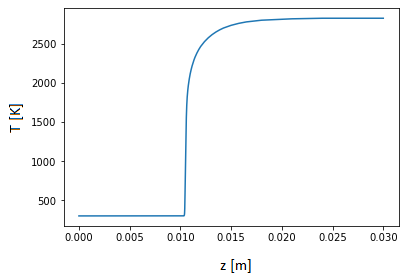
\includegraphics[height=0.5\textwidth]{P10}
        \caption{T (z) plot for Tint=300K, pint=1 atm, fi = 0,5.}
    \end{center}
\end{figure}

\begin{figure} [H]
	\begin{center}
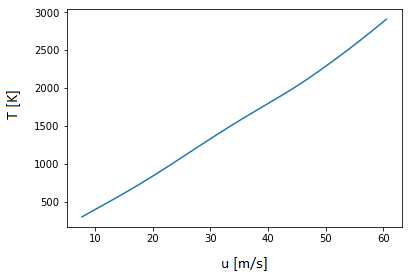
\includegraphics[height=0.5\textwidth]{P11}
        \caption{T (u) plot for Tint = 300K, pint = 1 atm, fi = 2.}
    \end{center}
\end{figure}

\begin{figure} [H]
	\begin{center}
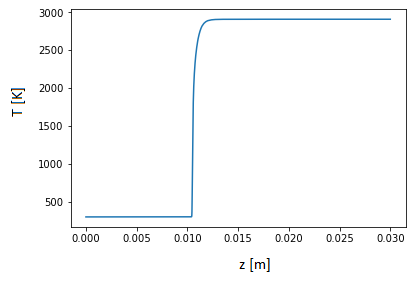
\includegraphics[height=0.5\textwidth]{P12}
        \caption{T (z) plot for Tint = 300K, pint = 1 atm, fi =2.}
    \end{center}
\end{figure}
Plot 1 and 2 show the calculations for Tint and pint. Plot 3 and 4 show the difference between Tint = 300K and Tint= 800K, as we see the velocity is higher in higher initial temperature case.  The calculation result is the same as in experiment provided in References. The higher initial temperature results in higher belocity, the shape and temperature of the flame is the same in both cases.Plot 5 and 6 show the calculations for Tint = 300K and pint = 0,1 atm. There are some differences in the velocity of the flame. The velocity is much lower in lower pressure than I basic. The shape of flame is different too. The temperature of the flame during the combustion is lower. Plot 7 and 8 show the calculations for Tint = 800K and pint = 0,1 atm. These plots show the differences between the previous  calculations with only one parameter which was changed. Plots 8-12 show the influence of different stoichiometry ratio (compared with plot 1 and 2 [fi = 1]).//
[2mm]
All provided results seem to be correct with the following References.


\section{References}
\begin{enumerate}
	\item{CANTERA\_HandsOn.pdf}
    \item{Wyklad\_4\_Cantera.pdf}
    \item{'Numerical study of geometric parameters effecting temperature and thermal efficiency in a premix multi-hole flat flame burner'  Mohammad Hossein Saberi Moghaddam, Mojtaba Saei Moghaddam, Mohammad Khorramdel,}
    \item{'Numerical investigation of pressure and temperature influence on flame speed CH2-H2 premixed combustion'  Punit Kumar, P. Anil Kishan, Atul Dhar,}
    \item{'Measurements of flat-flame velocities of diethyl ether in air' Fiona Gillespie, Wayne K. Metcalfe, Patricia Dirrenberger,}
    \item{'Numerical study of pressure influence on methane-oxygen laminar counterflow diffusion flames' Kimio Ilno, Fumiteru Akamatsu, Masashi Katsuki}
\end{enumerate}










\end{document}